\section{Results}\label{sec:results}
The results distinguish exact formulation agreement, availability, numerical
acceptance and elapsed-time inference. Tables~\ref{tab:catalog-1} and
\ref{tab:catalog-2} report every stored case/method outcome, including
incompatible cells. Objectives are compared within one unchanged model;
their numerical values are not ranked across different physical objectives.
Hard errors are evaluated on original rows, and N/A denotes the absence
of a compatible returned objective. The complete six-path timing comparison
and separate nine-policy grouped study have their own larger inventories.
\begin{table}[htbp]\centering\footnotesize
\caption{Complete stored catalog outcomes for the indicated cases and every catalog method. N/A means no compatible returned objective, and hard error is evaluated in original row coordinates.}\label{tab:catalog-1}
\begin{tabularx}{\textwidth}{@{}ll>{\raggedright\arraybackslash}Xrrr@{}}\toprule
Case & Method & State & Objective & Hard error & Gap\\\midrule
C01 & lifted & available & -2.\allowbreak{}98167 & 0 & 0\\
C01 & generalized & available & -2.\allowbreak{}98167 & 0 & 0\\
C01 & asymmetric & available & -2.\allowbreak{}98167 & 0 & 0\\
C01 & daqp & available & -2.\allowbreak{}98167 & 0 & 4.\allowbreak{}44089e-16\\
C02 & lifted & available & -2.\allowbreak{}98167 & 0 & 0\\
C02 & generalized & available & -2.\allowbreak{}98167 & 0 & 0\\
C02 & asymmetric & available & -2.\allowbreak{}98167 & 0 & 0\\
C02 & daqp & available & -2.\allowbreak{}98167 & 0 & 4.\allowbreak{}44089e-16\\
C03 & lifted & available & -2.\allowbreak{}564 & 0 & 0\\
C03 & generalized & incompatible & N/\allowbreak{}A & N/\allowbreak{}A & N/\allowbreak{}A\\
C03 & asymmetric & available & -2.\allowbreak{}564 & 0 & 4.\allowbreak{}44089e-16\\
C03 & daqp & available & -2.\allowbreak{}564 & 0 & 4.\allowbreak{}44089e-16\\
C04 & lifted & available & -4.\allowbreak{}14062 & 7.\allowbreak{}33857e-13 & 0\\
C04 & generalized & incompatible & N/\allowbreak{}A & N/\allowbreak{}A & N/\allowbreak{}A\\
C04 & asymmetric & available & -4.\allowbreak{}14063 & 6.\allowbreak{}95773e-10 & 9.\allowbreak{}57696e-11\\
C04 & daqp & available & -4.\allowbreak{}14062 & 0 & 1.\allowbreak{}01252e-13\\
C05 & lifted & available & -4.\allowbreak{}5 & 0 & 0\\
C05 & generalized & available & -4.\allowbreak{}5 & 0 & 2.\allowbreak{}66454e-15\\
C05 & asymmetric & incompatible & N/\allowbreak{}A & N/\allowbreak{}A & N/\allowbreak{}A\\
C05 & daqp & incompatible & N/\allowbreak{}A & N/\allowbreak{}A & N/\allowbreak{}A\\
C06 & lifted & available & -30.\allowbreak{}6139 & 0 & 0\\
C06 & generalized & incompatible & N/\allowbreak{}A & N/\allowbreak{}A & N/\allowbreak{}A\\
C06 & asymmetric & available & -30.\allowbreak{}6139 & 0 & 3.\allowbreak{}66003e-07\\
C06 & daqp & available & -30.\allowbreak{}6139 & 0 & 8.\allowbreak{}1416e-07\\
C07 & lifted & available & -34.\allowbreak{}5757 & 0 & 0\\
C07 & generalized & incompatible & N/\allowbreak{}A & N/\allowbreak{}A & N/\allowbreak{}A\\
C07 & asymmetric & available & -34.\allowbreak{}5757 & 0 & 1.\allowbreak{}09511e-07\\
C07 & daqp & incompatible & N/\allowbreak{}A & N/\allowbreak{}A & N/\allowbreak{}A\\
C08 & lifted & available & -2.\allowbreak{}64164 & 0 & 0\\
C08 & generalized & incompatible & N/\allowbreak{}A & N/\allowbreak{}A & N/\allowbreak{}A\\
C08 & asymmetric & available & -2.\allowbreak{}64164 & 0 & 1.\allowbreak{}24144e-08\\
C08 & daqp & available & -2.\allowbreak{}64164 & 0 & 1.\allowbreak{}32642e-08\\
\bottomrule\end{tabularx}
\end{table}

\begin{table}[htbp]\centering\footnotesize
\caption{Complete stored catalog outcomes for the indicated cases and every catalog method. N/A means no compatible returned objective, and hard error is evaluated in original row coordinates.}\label{tab:catalog-2}
\begin{tabularx}{\textwidth}{@{}ll>{\raggedright\arraybackslash}Xrrr@{}}\toprule
Case & Method & State & Objective & Hard error & Gap\\\midrule
C09 & lifted & available & -34.\allowbreak{}0702 & 0 & 0\\
C09 & generalized & available & -34.\allowbreak{}0702 & 9.\allowbreak{}42717e-08 & 2.\allowbreak{}83169e-07\\
C09 & asymmetric & available & -34.\allowbreak{}0702 & 9.\allowbreak{}42717e-08 & 2.\allowbreak{}83169e-07\\
C09 & daqp & available & -34.\allowbreak{}0702 & 8.\allowbreak{}88178e-16 & 6.\allowbreak{}51837e-09\\
C10 & lifted & available & -31.\allowbreak{}3247 & 0 & 0\\
C10 & generalized & available & -31.\allowbreak{}3247 & 1.\allowbreak{}82809e-07 & 8.\allowbreak{}24346e-07\\
C10 & asymmetric & available & -31.\allowbreak{}3247 & 1.\allowbreak{}82809e-07 & 8.\allowbreak{}24346e-07\\
C10 & daqp & available & -31.\allowbreak{}3247 & 1.\allowbreak{}77636e-15 & 1.\allowbreak{}03659e-08\\
C11 & lifted & available & 3.\allowbreak{}89929 & 0 & 0\\
C11 & generalized & incompatible & N/\allowbreak{}A & N/\allowbreak{}A & N/\allowbreak{}A\\
C11 & asymmetric & available & 3.\allowbreak{}89929 & 0 & 4.\allowbreak{}44089e-16\\
C11 & daqp & available & 3.\allowbreak{}89929 & 0 & 0\\
C12 & lifted & available & -41.\allowbreak{}204 & 1.\allowbreak{}90152e-10 & 0\\
C12 & generalized & incompatible & N/\allowbreak{}A & N/\allowbreak{}A & N/\allowbreak{}A\\
C12 & asymmetric & available & -41.\allowbreak{}204 & 4.\allowbreak{}21994e-10 & 4.\allowbreak{}61511e-08\\
C12 & daqp & available & -41.\allowbreak{}204 & 8.\allowbreak{}88178e-16 & 6.\allowbreak{}16883e-08\\
C13 & lifted & available & 36.\allowbreak{}6605 & 6.\allowbreak{}53606e-10 & 0\\
C13 & generalized & available & 36.\allowbreak{}6605 & 7.\allowbreak{}52559e-09 & 1.\allowbreak{}61722e-08\\
C13 & asymmetric & incompatible & N/\allowbreak{}A & N/\allowbreak{}A & N/\allowbreak{}A\\
C13 & daqp & incompatible & N/\allowbreak{}A & N/\allowbreak{}A & N/\allowbreak{}A\\
C14 & lifted & available & 48.\allowbreak{}403 & 2.\allowbreak{}37126e-09 & 0\\
C14 & generalized & incompatible & N/\allowbreak{}A & N/\allowbreak{}A & N/\allowbreak{}A\\
C14 & asymmetric & available & 48.\allowbreak{}403 & 2.\allowbreak{}09591e-08 & 2.\allowbreak{}54563e-06\\
C14 & daqp & incompatible & N/\allowbreak{}A & N/\allowbreak{}A & N/\allowbreak{}A\\
C15 & lifted & available & 42.\allowbreak{}6822 & 1.\allowbreak{}43467e-09 & 0\\
C15 & generalized & incompatible & N/\allowbreak{}A & N/\allowbreak{}A & N/\allowbreak{}A\\
C15 & asymmetric & available & 42.\allowbreak{}6822 & 2.\allowbreak{}72591e-09 & 2.\allowbreak{}17369e-06\\
C15 & daqp & incompatible & N/\allowbreak{}A & N/\allowbreak{}A & N/\allowbreak{}A\\
\bottomrule\end{tabularx}
\end{table}


Figure~\ref{fig:scalar-objective} isolates the scalar lower-side example.
The actual exported optima agree on a purchased lower departure rather than
on the preferred interval itself. Its piecewise-quadratic objective curve is an evaluation
of the stored mathematical objective, not an extra numerical experiment.
The shaded interval identifies preference, not a physical hard bound. This
small example illustrates why an elastic optimum can be correct while
violating the preferred row. Figure~\ref{fig:formulation-size} shows the
exported variable counts across all fifteen cases. Larger or smaller principal
formulations do not directly measure factorization fill, cache behavior or
complete-operation cost.
\begin{figure}[htbp]\centering
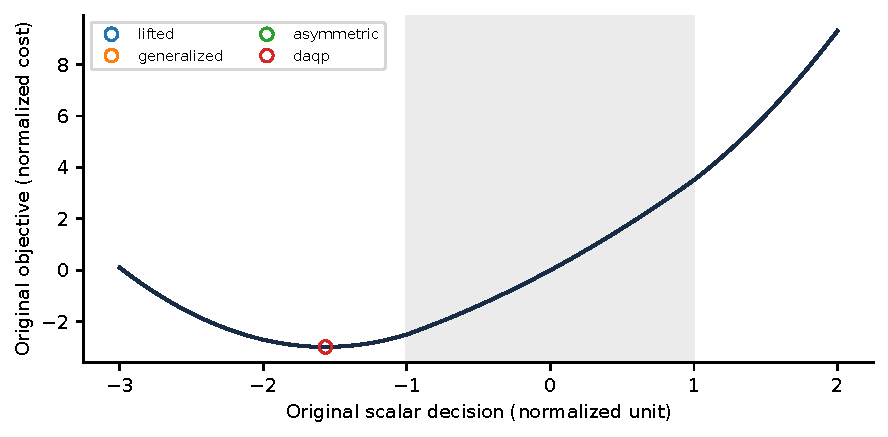
\includegraphics[width=.94\textwidth]{figures/scalar-objective.pdf}
\caption{Analytic evaluation of the stored C01 objective and actual exported method optima. The shaded interval is the preferred band, and the curve is a mathematical illustration rather than a new timed observation.}\label{fig:scalar-objective}
\end{figure}

\begin{figure}[htbp]\centering
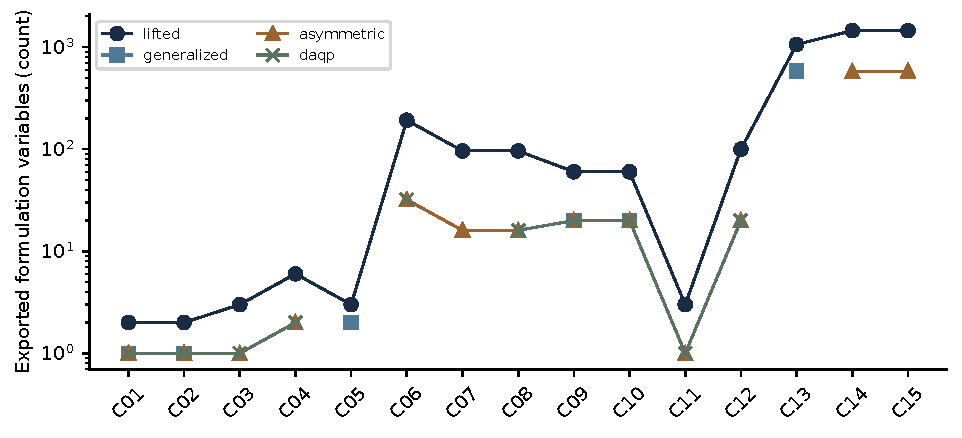
\includegraphics[width=.94\textwidth]{figures/formulation-size.pdf}
\caption{Exported variable counts for all fifteen stored catalog cases and four catalog paths. Missing points denote unsupported objectives; the counts describe formulation size and do not measure factorization fill or computational advantage.}\label{fig:formulation-size}
\end{figure}


Figure~\ref{fig:compatibility} makes the catalog's semantic exclusions explicit.
The source-faithful building objective admits lifting and published generalized
projection while refusing unsupported separable substitutions. The asymmetric
energy variants instead define different prices, so their stored objectives
cannot be read as algorithmic improvements over the mixed-policy optimum.
Likewise, an incompatible symmetric projection on the asymmetric C12 stream
is not a failed numerical solve of the same admitted objective. The matrix
distinguishes these states before any runtime reading is attempted.
\begin{figure}[htbp]\centering
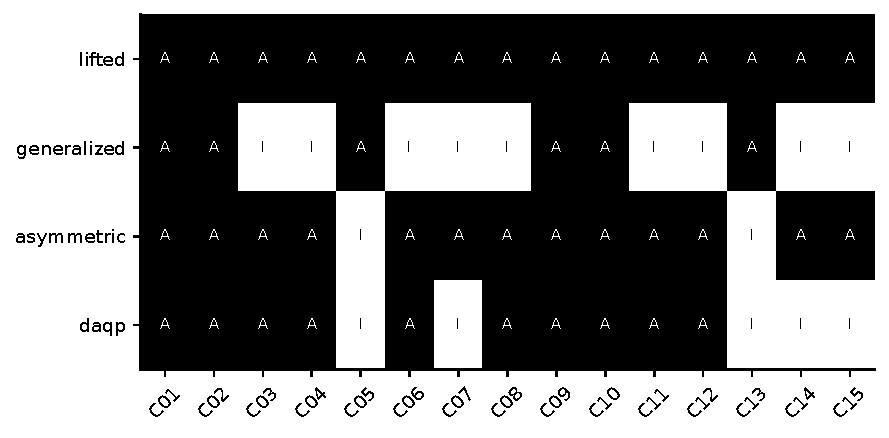
\includegraphics[width=.94\textwidth]{figures/compatibility.pdf}
\caption{Full catalog method-case compatibility: A denotes an available exported solution and I an incompatible requested objective. This four-path catalog is distinct from the six-path original timing study and the separate grouped study.}\label{fig:compatibility}
\end{figure}


The original computation completed all 456 planned instances with 11592 accepted
and 7560 incompatible measured observations and no numerical or external-accuracy
rejection. Table~\ref{tab:main-results} preserves its primary 168 paired
observations and the separate grouped endpoint. The original reduction
\OriginalEstimate\% has a 95\% interval crossing zero. Figure~\ref{fig:original-effect}
therefore does not establish the predicted 10\% gain. The plotted zero and
ten-percent reference lines are inferential context, not replacement cutoffs
chosen after observing the estimate. Figure~\ref{fig:cold-times} shows stored
cell medians and interquartile ranges for one prespecified family/density
slice; that descriptive slice does not replace the full primary analysis.
\begin{table}[htbp]\centering\footnotesize
\caption{Distinct primary populations, stored effect estimates and uncertainty for the two completed timing studies. Failed-pair rules are not transferred between experiments and neither registered ten percent improvement criterion is established.}\label{tab:main-results}
\begin{tabularx}{\textwidth}{@{}>{\raggedright\arraybackslash}Xrrrr@{}}\toprule
Study & Population & Pairs & Effect (\%) & 95\% limits\\\midrule
Separable & 456 & 168 & 0.\allowbreak{}499839 & -3.\allowbreak{}29197, 3.\allowbreak{}94484\\
Grouped & 210 & 144 & -212.\allowbreak{}45 & -225.\allowbreak{}337, -192.\allowbreak{}874\\
\bottomrule\end{tabularx}
\end{table}

\begin{figure}[htbp]\centering
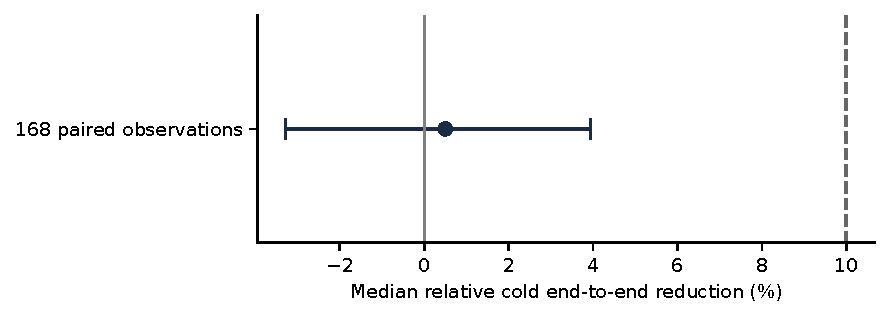
\includegraphics[width=.94\textwidth]{figures/original-effect.pdf}
\caption{Original held-out timing estimate with its stored 95 percent seed-cluster confidence interval and registered ten percent reference. The interval crosses zero; neither interval nor population is recomputed for this figure.}\label{fig:original-effect}
\end{figure}

\begin{figure}[htbp]\centering
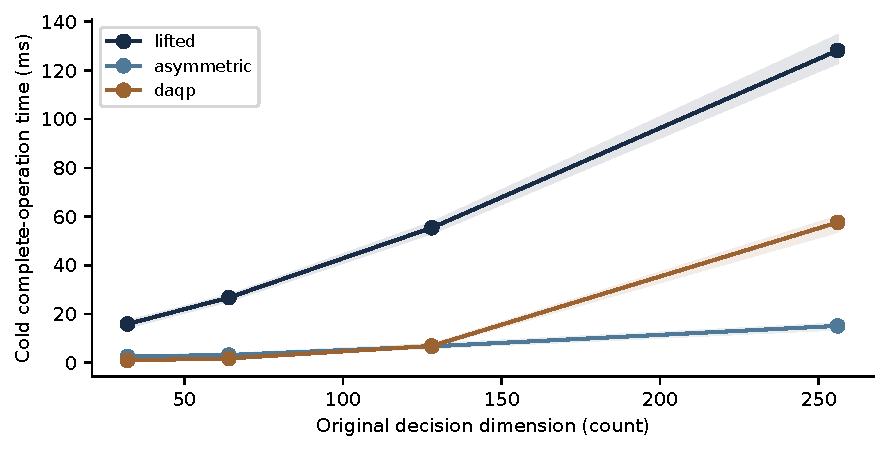
\includegraphics[width=.94\textwidth]{figures/cold-times.pdf}
\caption{Stored held-out asymmetric-elastic timing cells at density 0.05 and unit diagonal condition. Lines are stored medians and bands stored interquartile ranges; this descriptive subset does not replace the complete primary endpoint.}\label{fig:cold-times}
\end{figure}


The controlled conditioning results in Figure~\ref{fig:conditioning} retain
maximum objective discrepancy for each compatible robustness cell. The
finite grid extends to diagonal condition$10^6$, and its accepted observations
remain within the original objective and hard-row limits. The plot does not
establish stability for arbitrary nearly dependent rows, every semidefinite
problem, or an untested physical scaling. A missing method remains absent,
not an invented zero-error point. Relative objective agreement also does
not prove an identical dual vector when the mathematical dual is nonunique.
\begin{figure}[htbp]\centering
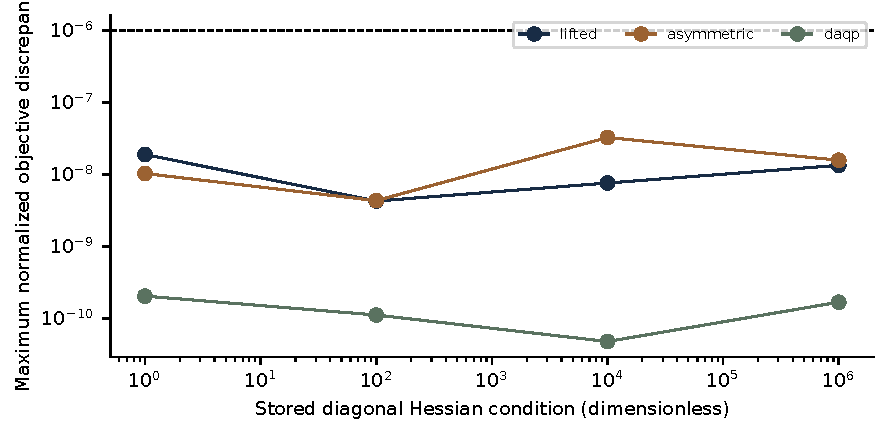
\includegraphics[width=.94\textwidth]{figures/conditioning.pdf}
\caption{Maximum stored objective discrepancy in each compatible robustness cell by diagonal condition. The dashed line is the original external objective criterion; absent methods remain absent rather than receiving an invented zero discrepancy.}\label{fig:conditioning}
\end{figure}


The common trajectory in Figure~\ref{fig:control-stream} shows the actual
stored position, velocity and bounded applied acceleration. It is driven
once by the independent oracle. Figure~\ref{fig:stream-reuse} compares stored
cold and warm operation durations along those same inputs. Workspace reuse
can reduce preparation work, but the stream alone cannot attribute every
timing difference solely to an active set, initial iterate or cached factor.
The plotted box summaries describe the retained observations; they are not
a new cluster-bootstrap experiment. Overlapping predicted horizon costs
remain distinct from realized plant cost.
\begin{figure}[htbp]\centering
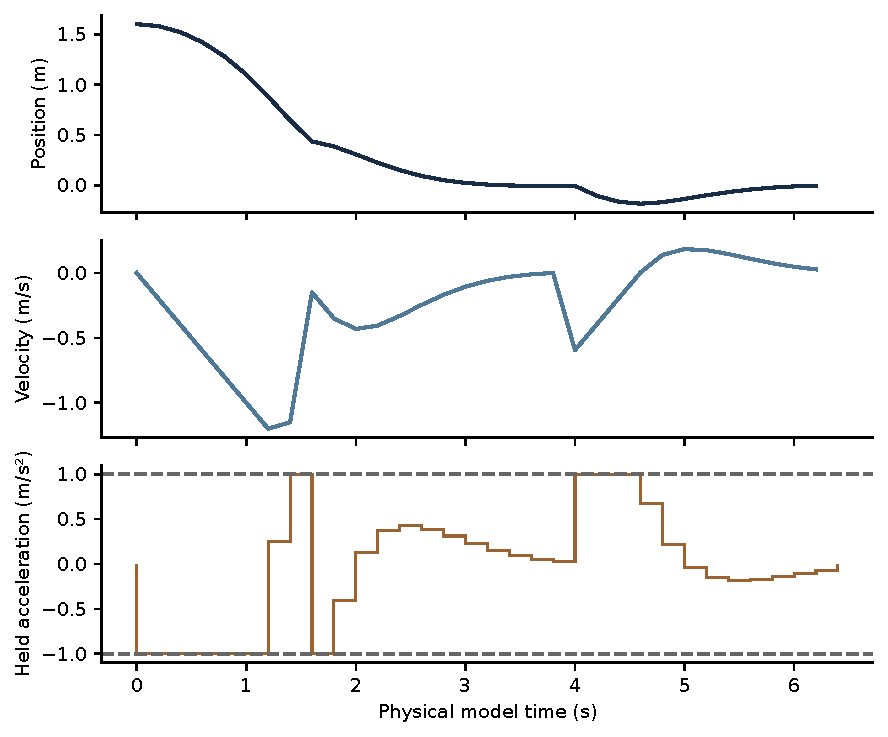
\includegraphics[width=.94\textwidth]{figures/control-stream.pdf}
\caption{The stored common C12 plant trajectory and interval-held oracle acceleration across thirty-two frames. Steps retain each complete physical sampling interval; these curves are not separate closed-loop controller performance measurements.}\label{fig:control-stream}
\end{figure}

\begin{figure}[htbp]\centering
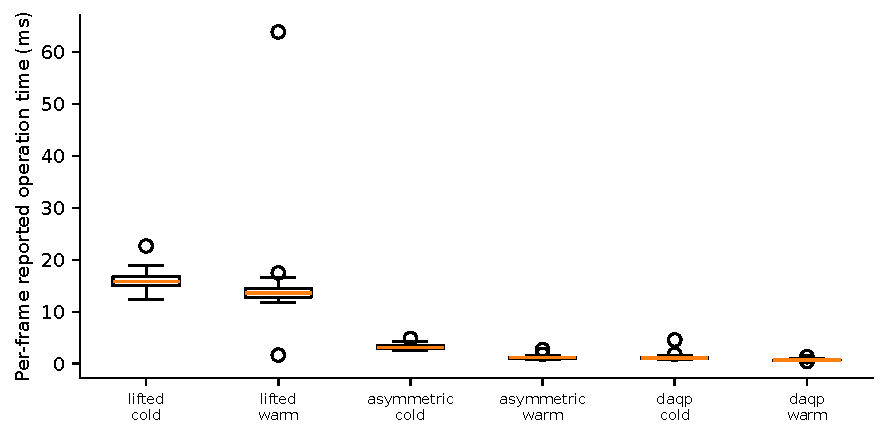
\includegraphics[width=.94\textwidth]{figures/stream-reuse.pdf}
\caption{Stored cold and warm C12 operation durations for every accepted frame of each compatible method. The box summaries are descriptive paired-path evidence, not a randomized causal isolation of warm starting from all other implementation choices.}\label{fig:stream-reuse}
\end{figure}


The grouped computation retains all 210 inputs. Table~\ref{tab:coupled-states}
and Figure~\ref{fig:coupled-states} account for all 5670 measured method
observations:3667 accepted,12 accuracy-rejected,1719 incompatible,270 dependent
oracle-failed and two timeouts. The larger raw inventory additionally retains
warm-ups and oracle observations. All 163390 returned candidate frames pass
their applicable original-space checks;44 noncandidate backend-limit frames
remain distinct. Those frame checks do not turn an iteration-limited batch
into an accepted primary operation.

The accuracy-rejected category must not be read as twelve returned
vectors violating the independent KKT calculation. The retained batches
include backend/iteration-limit or absent-vector outcomes; in particular,
six held-out row-split batches returned status seven without a candidate
vector. The two timeouts occurred in native and forced-proximal DAQP
operations. Six robustness oracle limits account for the dependent
144 measured oracle-failed rows in that split. These are operation and
dependency states, not additional independent KKT violations. Every
returned candidate frame still passed the applicable original-space checks.
\begin{table}[htbp]\centering\footnotesize
\caption{Measured grouped-study method states by split, including dependent oracle failures and supervised timeouts. Counts cover all measured method rows, while warm-up and oracle observations remain in the larger raw archive.}\label{tab:coupled-states}
\begin{tabularx}{\textwidth}{@{}>{\raggedright\arraybackslash}Xrrrrr@{}}\toprule
Split & Accepted & Accuracy & Incompat. & Oracle & Timeout\\\midrule
development & 879 & 0 & 396 & 21 & 0\\
heldout & 2587 & 6 & 1188 & 105 & 2\\
robustness & 201 & 6 & 135 & 144 & 0\\
\bottomrule\end{tabularx}
\end{table}

\begin{figure}[htbp]\centering
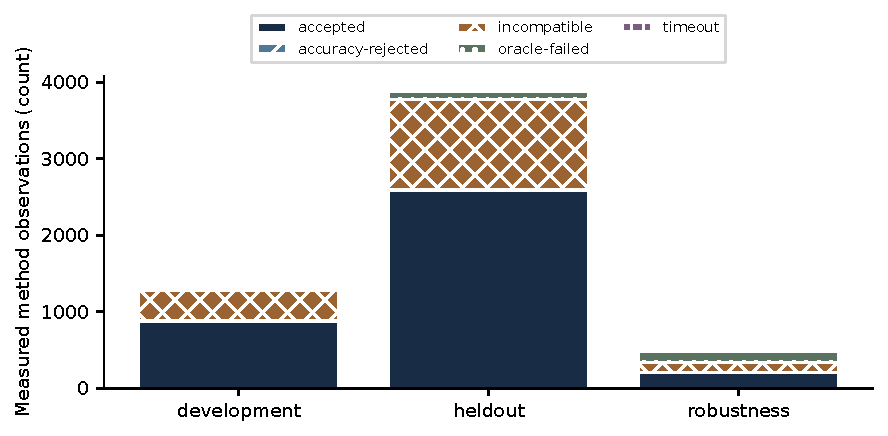
\includegraphics[width=.94\textwidth]{figures/coupled-states.pdf}
\caption{All 5670 measured method observations of the grouped study, separated by their original development, held-out and robustness splits. Acceptance, accuracy rejection, incompatibility, dependent oracle failure and supervised timeout remain different categories.}\label{fig:coupled-states}
\end{figure}


Figure~\ref{fig:coupled-population} retains all 144 primary members in their
stored order. Nine failed pairs keep their fixed score, and six missing
native medians remain gaps. No selected baseline is imputed where the
registered rule selected none. The primary median reduction is
\PrimaryEstimate\%, with 95\% limits \PrimaryLower\% and \PrimaryUpper\%.
These values do not define a uniform per-instance slowdown multiplier.
Figure~\ref{fig:coupled-formulations} displays returned method medians with
their unequal sample counts. It is a descriptive formulation comparison,
not an alternative matched estimator that removes failures or compatibility
differences. The original primary prediction is not rescued by those plots.
\begin{figure}[htbp]\centering
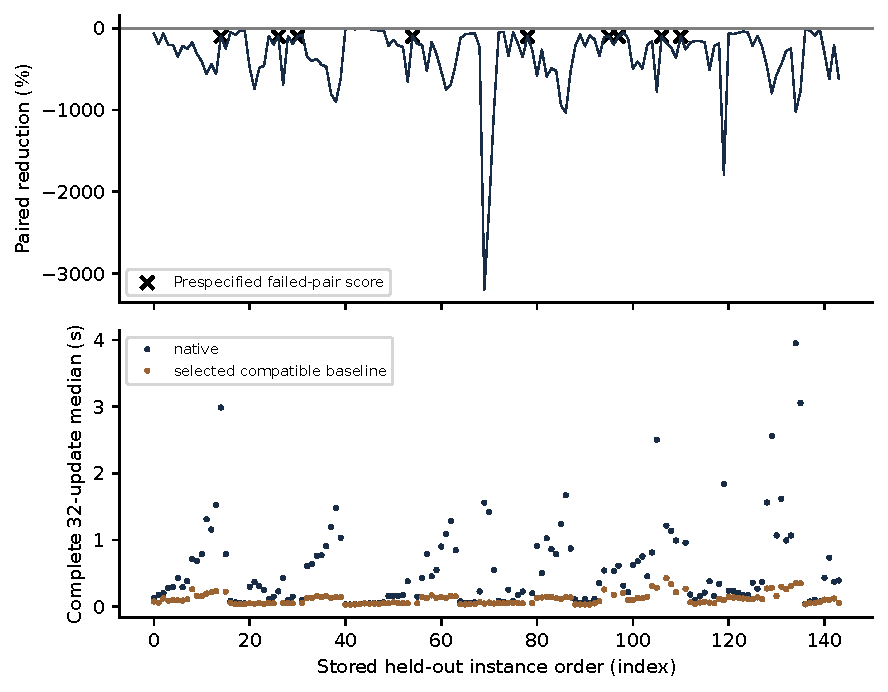
\includegraphics[width=.94\textwidth]{figures/coupled-population.pdf}
\caption{All 144 stored grouped-study primary members in original order, with nine failed scores retained. Complete-operation medians preserve missing values as gaps and do not impute a comparator where the primary rule selected none.}\label{fig:coupled-population}
\end{figure}

\begin{figure}[htbp]\centering
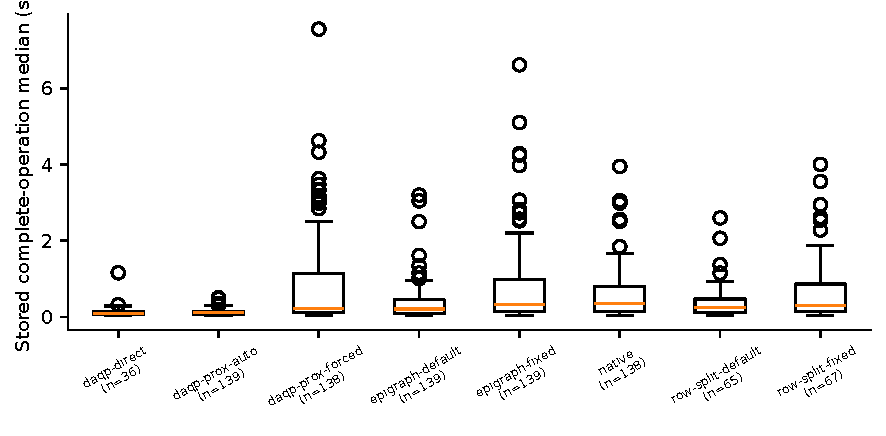
\includegraphics[width=.94\textwidth]{figures/coupled-formulations.pdf}
\caption{Distributions of stored held-out per-instance medians for each returned compatible formulation. Sample counts differ because compatibility and failures differ; these unmatched descriptive distributions are not the registered paired comparison or a causal ablation.}\label{fig:coupled-formulations}
\end{figure}


Finally, Figure~\ref{fig:directional-lesson} gives the stored native, epigraph
and directional row-split answers for the same two-variable physical teaching
input. Their objective and decision agreement illustrates representation
equivalence on a transparent example. It contributes no new timing sample
to either registered study. The dimensional covariance checks and policy
scale changes described in the teaching material distinguish preserving
physical meaning from intentionally changing a directional preference.
The coexistence of that numerical agreement with the complete negative
timing endpoint is the principal practical result: mathematical equivalence
and smaller principal dimensions do not guarantee a cheaper complete operation.
\begin{figure}[htbp]\centering
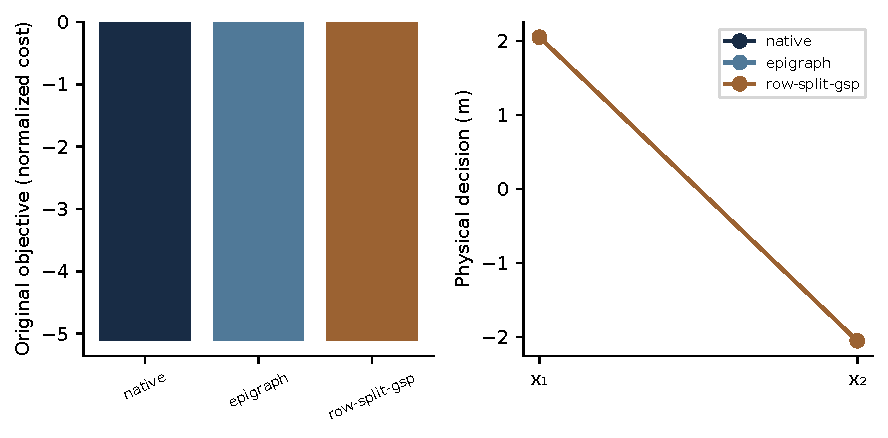
\includegraphics[width=.94\textwidth]{figures/directional-lesson.pdf}
\caption{Stored native, epigraph and directional row-split answers for the same two-variable physical teaching input. Objective and decision agreement are a small numerical illustration, not additional timing evidence or an independent experiment.}\label{fig:directional-lesson}
\end{figure}

